\documentclass[11pt]{article}
\usepackage{amsmath}
\usepackage{amssymb}
\usepackage{graphicx} % Required for inserting images
\usepackage{hyperref}
\usepackage{enumitem}
\usepackage{xcolor}
\usepackage{booktabs}
\usepackage{multirow}
\usepackage{subcaption,wrapfig}
\title{The Solar System}
\author{Johanes Kepler$^1$}
\date{
\small
$^1$ Imperial Mathematician,Prague
}

\begin{document}

\maketitle

\section{Our Planetary Neighbourhpod}
\subsection{The Sun and Its Planets}
The Sun and its gravity-bounded bodies from the Solar Systems\cite{kepler1609}.\footnote{Sizes and distances are schematic}See \href{https://science.nasa.gov/}{Nasa Solar Sysetm exploration}.In increasing distance, the planets are \\
Mercury, Venus, Earth, Mars, Jupiter, Saturn, Uranus, Neptune.\\
The planets form two groups:
\begin{enumerate}[label=(\Roman*)]
    \item Inner Planets
    \begin{itemize}[label=\textdagger]
        \item Mercury earcth and venus
        \item they are compaarvely
        \item they are alsoc alled
    \end{itemize}
    \item Outer Plannets
        \begin{itemize}[label=\textdagger]
        \item Jupyter nd  Saturn are
        \item Uranus are Neptune
        \item All four outer 
    \end{itemize}
\end{enumerate}

\textcolor{blue}{The inner planets are small, dense, and relatively close to the Sun, }whereas
\textcolor{red}{the outer planets are much larger and travel along considerably wider orbits.}

\subsection{Portraits of the Solar System}
Figure 1 shows the Sun and eight planets.1
Compare Mars in Figure 1e with Jupiter in Figure 1f.

\section{Kepler’s Laws of Planetary Motion}
Kepler’s three laws describe planetary motion \cite{nasa_kepler}. The first law describes the shape of planetary orbits, the second law describes the speed of planetary motion, and the third law relates the orbital period to the size of the orbit.
\subsection{First Law: Elliptical Orbits}
A planetary orbit is elliptical, with the Sun at one focus:
\begin{equation}
    \frac{x^{2}}{a^{2}} + \frac{y^{2}}{b^{2}} =1 , a \ge b > 0,
\end{equation}
Here a and b are the semi-axes.
For focal distance c,
\begin{align}
    c^{2} &= a^{2} - b^{2} \notag \\
    e &= \frac{c}{a}
\end{align}
Here e is the eccentricity.\\
In polar form,
\begin{equation}
    r(\theta) = \frac{a(1-e^{2}) }{1+e\cos\theta}.
    \label{eq:big}
\end{equation}
Equation \hyperref[eq:big]{(3)} gives the orbital distance.

\subsection{Second Law: Equal Areas in Equal Times}
Equal times sweep equal areas:
\begin{equation}
    \Delta t_{1} =\Delta t_{2} \implies \Delta A_{1} =\Delta A_{2}
\end{equation}
Consequently, a planet moves
\begin{itemize}[label=$\diamond$]
    \item faster when
    \item slower when
\end{itemize}

\subsection{Third Law: Orbital Period and Distance}
For planets orbiting one star,
\begin{equation}
    T^{2} \propto a^{3}
\end{equation}
Newtoninan form:
\begin{equation}
    T^{2} = \frac{4 \pi^{2}}{GM_{.}}a^{3} \notag
\end{equation}
Here $M_{.}$ is the solar mass.

\subsection{An Earth–Mars Comparison}
Using Earth as reference,
$a_{E} = 1 AU ; T_{E} = 1 year $





\section{ The Outer Planets}
The outer planets are Jupiter, Saturn, Uranus, and Neptune \cite{nasa_temperatures}. The first two
are \textit{gas giants}; the last two are \textit{ice giants}.\\
Table 1 uses scientific and relativistic notation.\footnote{Values are rounded for typesetting practice.}
\begin{table}[h]
    \centering
    \caption{Orbital and Relativistic Parameters}
    \label{tab:placeholder}
    \begin{tabular}{lcccc}
        \toprule
        \multirow{2}{*}{Planets} & \multicolumn{2}{c}{Orbital Parameters} & \multicolumn{2}{c}{Relativistic Motion}\\
        \cmidrule(lr){2-3} \cmidrule(lr){4-5}
        & $a$ (AU) & $e$ & $\epsilon = \frac{1}{ac^{2}}GM$ & $\beta= \sqrt{\epsilon}$ \\
        \midrule
        Jupiter & 5.204 & 0.0489 & 0.000 & 0.000 \\
        Saturn & 9.582 & 0.0565 & 0.000 & 0.000 \\
        Uranus & 19.201 & 0.0463 & 0.000 & 0.000 \\
        Neptune & 30.047 & 0.0097 & 0.000 & 0.000 \\
        \bottomrule
    \end{tabular}
\end{table}

Table \ref{tab:placeholder} compares the four giant planets.
\bibliographystyle{plain}
\bibliography{solar_system} \newpage
\section{Conclusion}
\begin{figure}[h]
    \centering
    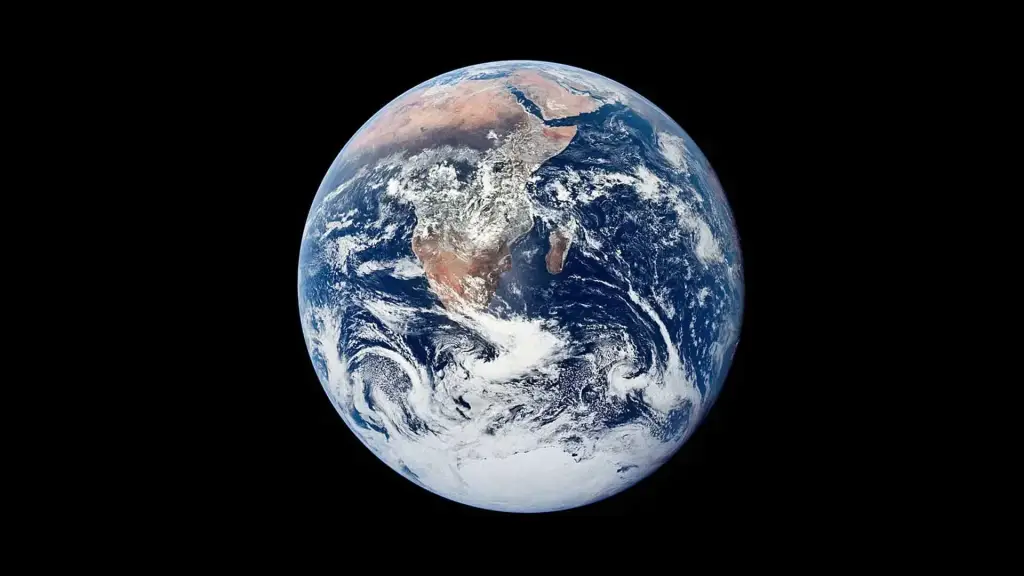
\includegraphics[width=0.8\textwidth]{earth.png}    
    \caption{The Sun and its planets.}
    \label{fig:earth}
\end{figure}


\begin{figure}[h]
    \centering
    \begin{subfigure}{0.3\textwidth}
        \centering
        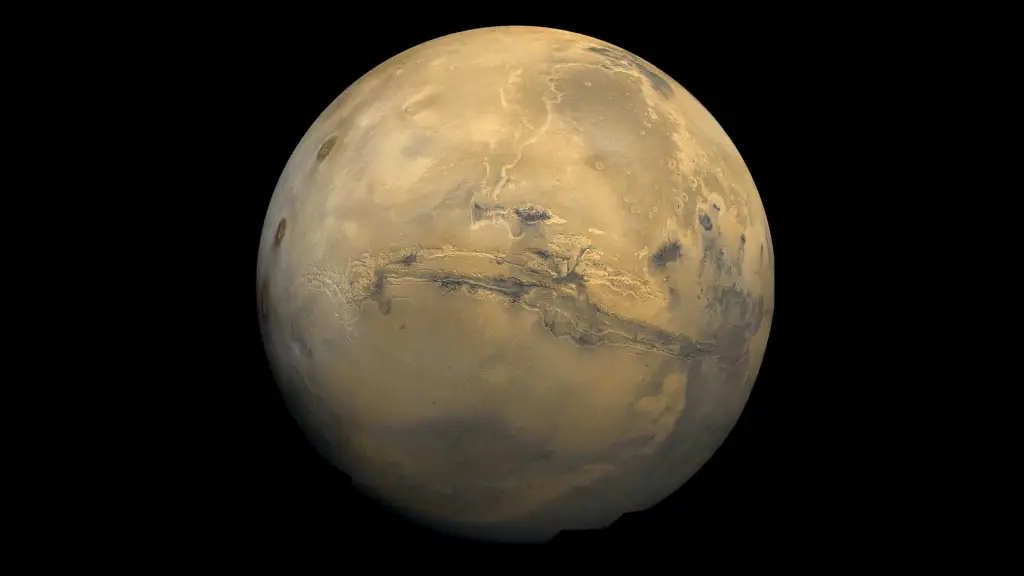
\includegraphics[width=\linewidth]{mars.png}
        \caption{Mars}
        \label{fig:mars}
    \end{subfigure} \hfill
     \begin{subfigure}{0.3\textwidth}
        \centering
        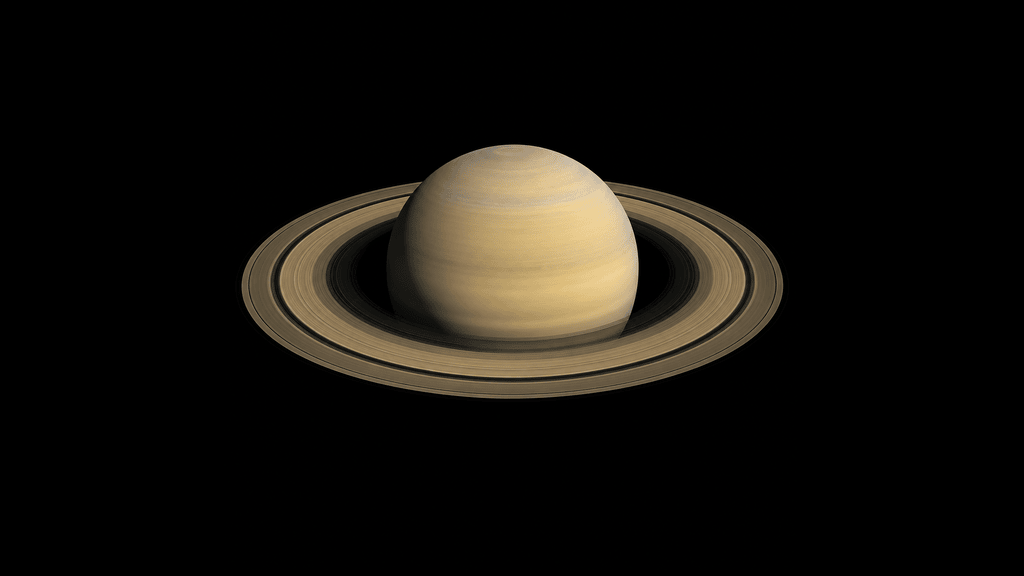
\includegraphics[width=\linewidth]{saturn.png}
        \caption{Saturn}
        \label{fig:saturn}
    \end{subfigure} \hfill
    \begin{subfigure}{0.3\textwidth}
        \centering
        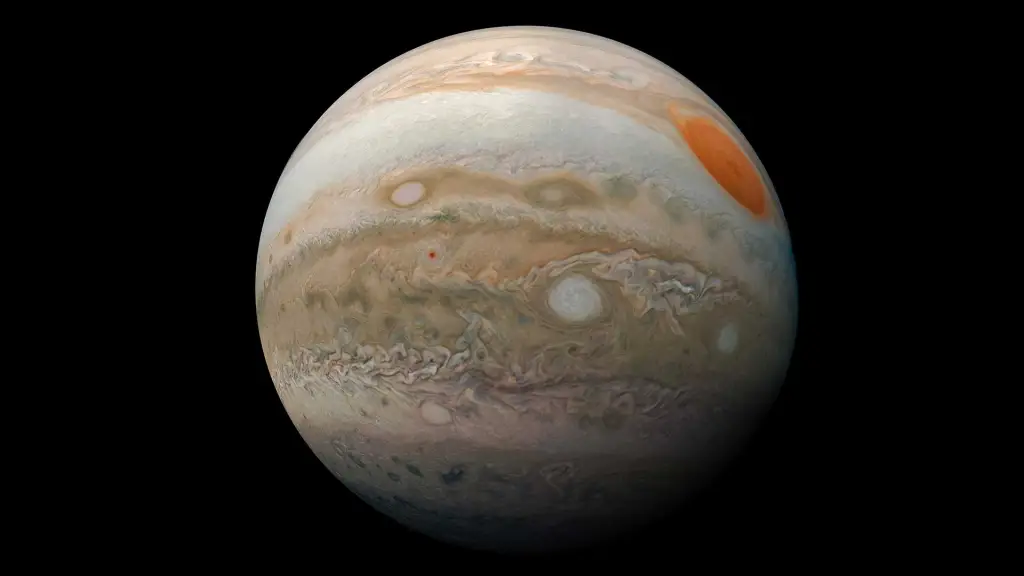
\includegraphics[width=\linewidth]{jupiter.png}
        \caption{Jupiter}
        \label{fig:jupiter}
    \end{subfigure}
\caption{two panels}
\end{figure}
\[
\mathcal{P} = \frac{1}{2}mv^{2} - \frac{GMm}{r} = -\frac{GMm}{2a}
\]
\end{document}
